\documentclass[11pt,]{article}
\usepackage{lmodern}
\usepackage{amssymb,amsmath}
\usepackage{ifxetex,ifluatex}
\usepackage{fixltx2e} % provides \textsubscript
\ifnum 0\ifxetex 1\fi\ifluatex 1\fi=0 % if pdftex
  \usepackage[T1]{fontenc}
  \usepackage[utf8]{inputenc}
\else % if luatex or xelatex
  \ifxetex
    \usepackage{mathspec}
    \usepackage{xltxtra,xunicode}
  \else
    \usepackage{fontspec}
  \fi
  \defaultfontfeatures{Mapping=tex-text,Scale=MatchLowercase}
  \newcommand{\euro}{€}
\fi
% use upquote if available, for straight quotes in verbatim environments
\IfFileExists{upquote.sty}{\usepackage{upquote}}{}
% use microtype if available
\IfFileExists{microtype.sty}{%
\usepackage{microtype}
\UseMicrotypeSet[protrusion]{basicmath} % disable protrusion for tt fonts
}{}
\usepackage[margin=1in]{geometry}
\ifxetex
  \usepackage[setpagesize=false, % page size defined by xetex
              unicode=false, % unicode breaks when used with xetex
              xetex]{hyperref}
\else
  \usepackage[unicode=true]{hyperref}
\fi
\hypersetup{breaklinks=true,
            bookmarks=true,
            pdfauthor={David J. Harris},
            pdftitle={Appendix 4: Results},
            colorlinks=true,
            citecolor=blue,
            urlcolor=blue,
            linkcolor=magenta,
            pdfborder={0 0 0}}
\urlstyle{same}  % don't use monospace font for urls
\usepackage{color}
\usepackage{fancyvrb}
\newcommand{\VerbBar}{|}
\newcommand{\VERB}{\Verb[commandchars=\\\{\}]}
\DefineVerbatimEnvironment{Highlighting}{Verbatim}{commandchars=\\\{\}}
% Add ',fontsize=\small' for more characters per line
\usepackage{framed}
\definecolor{shadecolor}{RGB}{248,248,248}
\newenvironment{Shaded}{\begin{snugshade}}{\end{snugshade}}
\newcommand{\KeywordTok}[1]{\textcolor[rgb]{0.13,0.29,0.53}{\textbf{{#1}}}}
\newcommand{\DataTypeTok}[1]{\textcolor[rgb]{0.13,0.29,0.53}{{#1}}}
\newcommand{\DecValTok}[1]{\textcolor[rgb]{0.00,0.00,0.81}{{#1}}}
\newcommand{\BaseNTok}[1]{\textcolor[rgb]{0.00,0.00,0.81}{{#1}}}
\newcommand{\FloatTok}[1]{\textcolor[rgb]{0.00,0.00,0.81}{{#1}}}
\newcommand{\ConstantTok}[1]{\textcolor[rgb]{0.00,0.00,0.00}{{#1}}}
\newcommand{\CharTok}[1]{\textcolor[rgb]{0.31,0.60,0.02}{{#1}}}
\newcommand{\SpecialCharTok}[1]{\textcolor[rgb]{0.00,0.00,0.00}{{#1}}}
\newcommand{\StringTok}[1]{\textcolor[rgb]{0.31,0.60,0.02}{{#1}}}
\newcommand{\VerbatimStringTok}[1]{\textcolor[rgb]{0.31,0.60,0.02}{{#1}}}
\newcommand{\SpecialStringTok}[1]{\textcolor[rgb]{0.31,0.60,0.02}{{#1}}}
\newcommand{\ImportTok}[1]{{#1}}
\newcommand{\CommentTok}[1]{\textcolor[rgb]{0.56,0.35,0.01}{\textit{{#1}}}}
\newcommand{\DocumentationTok}[1]{\textcolor[rgb]{0.56,0.35,0.01}{\textbf{\textit{{#1}}}}}
\newcommand{\AnnotationTok}[1]{\textcolor[rgb]{0.56,0.35,0.01}{\textbf{\textit{{#1}}}}}
\newcommand{\CommentVarTok}[1]{\textcolor[rgb]{0.56,0.35,0.01}{\textbf{\textit{{#1}}}}}
\newcommand{\OtherTok}[1]{\textcolor[rgb]{0.56,0.35,0.01}{{#1}}}
\newcommand{\FunctionTok}[1]{\textcolor[rgb]{0.00,0.00,0.00}{{#1}}}
\newcommand{\VariableTok}[1]{\textcolor[rgb]{0.00,0.00,0.00}{{#1}}}
\newcommand{\ControlFlowTok}[1]{\textcolor[rgb]{0.13,0.29,0.53}{\textbf{{#1}}}}
\newcommand{\OperatorTok}[1]{\textcolor[rgb]{0.81,0.36,0.00}{\textbf{{#1}}}}
\newcommand{\BuiltInTok}[1]{{#1}}
\newcommand{\ExtensionTok}[1]{{#1}}
\newcommand{\PreprocessorTok}[1]{\textcolor[rgb]{0.56,0.35,0.01}{\textit{{#1}}}}
\newcommand{\AttributeTok}[1]{\textcolor[rgb]{0.77,0.63,0.00}{{#1}}}
\newcommand{\RegionMarkerTok}[1]{{#1}}
\newcommand{\InformationTok}[1]{\textcolor[rgb]{0.56,0.35,0.01}{\textbf{\textit{{#1}}}}}
\newcommand{\WarningTok}[1]{\textcolor[rgb]{0.56,0.35,0.01}{\textbf{\textit{{#1}}}}}
\newcommand{\AlertTok}[1]{\textcolor[rgb]{0.94,0.16,0.16}{{#1}}}
\newcommand{\ErrorTok}[1]{\textcolor[rgb]{0.64,0.00,0.00}{\textbf{{#1}}}}
\newcommand{\NormalTok}[1]{{#1}}
\usepackage{longtable,booktabs}
\usepackage{graphicx,grffile}
\makeatletter
\def\maxwidth{\ifdim\Gin@nat@width>\linewidth\linewidth\else\Gin@nat@width\fi}
\def\maxheight{\ifdim\Gin@nat@height>\textheight\textheight\else\Gin@nat@height\fi}
\makeatother
% Scale images if necessary, so that they will not overflow the page
% margins by default, and it is still possible to overwrite the defaults
% using explicit options in \includegraphics[width, height, ...]{}
\setkeys{Gin}{width=\maxwidth,height=\maxheight,keepaspectratio}
\setlength{\parindent}{0pt}
\setlength{\parskip}{6pt plus 2pt minus 1pt}
\setlength{\emergencystretch}{3em}  % prevent overfull lines
\providecommand{\tightlist}{%
  \setlength{\itemsep}{0pt}\setlength{\parskip}{0pt}}
\setcounter{secnumdepth}{0}

%%% Use protect on footnotes to avoid problems with footnotes in titles
\let\rmarkdownfootnote\footnote%
\def\footnote{\protect\rmarkdownfootnote}

%%% Change title format to be more compact
\usepackage{titling}

% Create subtitle command for use in maketitle
\newcommand{\subtitle}[1]{
  \posttitle{
    \begin{center}\large#1\end{center}
    }
}

\setlength{\droptitle}{-2em}
  \title{Appendix 4: Results}
  \pretitle{\vspace{\droptitle}\centering\huge}
  \posttitle{\par}
\subtitle{Inferring species interactions from co-occurrence data with Markov
networks}
  \author{David J. Harris}
  \preauthor{\centering\large\emph}
  \postauthor{\par}
  \date{}
  \predate{}\postdate{}


% Redefines (sub)paragraphs to behave more like sections
\ifx\paragraph\undefined\else
\let\oldparagraph\paragraph
\renewcommand{\paragraph}[1]{\oldparagraph{#1}\mbox{}}
\fi
\ifx\subparagraph\undefined\else
\let\oldsubparagraph\subparagraph
\renewcommand{\subparagraph}[1]{\oldsubparagraph{#1}\mbox{}}
\fi

\begin{document}
\maketitle

\begin{Shaded}
\begin{Highlighting}[]
\KeywordTok{library}\NormalTok{(dplyr)}
\KeywordTok{library}\NormalTok{(mgcv)}
\KeywordTok{library}\NormalTok{(ggplot2)}
\KeywordTok{library}\NormalTok{(tidyr)}
\KeywordTok{library}\NormalTok{(knitr)}
\KeywordTok{library}\NormalTok{(lme4)}
\end{Highlighting}
\end{Shaded}

\subsection{Import the results from Appendix
4:}\label{import-the-results-from-appendix-4}

\begin{Shaded}
\begin{Highlighting}[]
\NormalTok{x =}\StringTok{ }\KeywordTok{read.csv}\NormalTok{(}\StringTok{"estimates.csv"}\NormalTok{, }\DataTypeTok{stringsAsFactors =} \OtherTok{FALSE}\NormalTok{)}
\NormalTok{x$simulation_type =}\StringTok{ }\KeywordTok{gsub}\NormalTok{(}\StringTok{"[0-9]"}\NormalTok{, }\StringTok{""}\NormalTok{, x$rep_name)}
\end{Highlighting}
\end{Shaded}

\subsection{\texorpdfstring{Import the results from the \emph{Pairs}
software:}{Import the results from the Pairs software:}}\label{import-the-results-from-the-pairs-software}

\begin{Shaded}
\begin{Highlighting}[]
\NormalTok{pairs_txt =}\StringTok{ }\KeywordTok{readLines}\NormalTok{(}\StringTok{"fakedata/matrices/Pairs.txt"}\NormalTok{)}
\KeywordTok{library}\NormalTok{(stringr)}

\CommentTok{# Find areas of the data file that correspond}
\CommentTok{# to species pairs' results}
\NormalTok{beginnings =}\StringTok{ }\KeywordTok{grep}\NormalTok{(}\StringTok{"Sp1"}\NormalTok{, pairs_txt) +}\StringTok{ }\DecValTok{1}
\NormalTok{ends =}\StringTok{ }\KeywordTok{c}\NormalTok{(}
  \KeywordTok{grep}\NormalTok{(}\StringTok{"^[^ ]"}\NormalTok{, pairs_txt)[-}\DecValTok{1}\NormalTok{],}
  \KeywordTok{length}\NormalTok{(pairs_txt) +}\StringTok{ }\DecValTok{1}
\NormalTok{) -}\StringTok{ }\DecValTok{1}

\NormalTok{partial_names =}\StringTok{ }\KeywordTok{sapply}\NormalTok{(}\KeywordTok{strsplit}\NormalTok{(}\KeywordTok{grep}\NormalTok{(}\StringTok{"^>"}\NormalTok{, pairs_txt, }\DataTypeTok{value =} \OtherTok{TRUE}\NormalTok{), }\StringTok{" +"}\NormalTok{), function(x) x[[}\DecValTok{3}\NormalTok{]])}
\NormalTok{filename_lines =}\StringTok{ }\KeywordTok{grep}\NormalTok{(}\StringTok{"^>"}\NormalTok{, pairs_txt)}

\CommentTok{# Sort a vector of alphanumeric strings by the numeric component}
\CommentTok{# as if they were integers.  For example, V20 is larger than V12,}
\CommentTok{# even though V12 comes first alphabetically}
\NormalTok{alnum_sort =}\StringTok{ }\NormalTok{function(x)\{}
  \NormalTok{raw =}\StringTok{ }\KeywordTok{as.integer}\NormalTok{(}\KeywordTok{gsub}\NormalTok{(}\StringTok{"[[:alpha:]]"}\NormalTok{, }\StringTok{""}\NormalTok{, x))}
  \NormalTok{x[}\KeywordTok{order}\NormalTok{(raw)]}
\NormalTok{\}}

\NormalTok{pairs_results =}\StringTok{ }\KeywordTok{lapply}\NormalTok{(}
  \DecValTok{1}\NormalTok{:}\KeywordTok{length}\NormalTok{(filename_lines),}
  \NormalTok{function(i)\{}
    
    \NormalTok{n_sites =}\StringTok{ }\KeywordTok{as.integer}\NormalTok{(}\KeywordTok{strsplit}\NormalTok{(partial_names[[i]], }\StringTok{"-"}\NormalTok{)[[}\DecValTok{1}\NormalTok{]][[}\DecValTok{1}\NormalTok{]])}
    \NormalTok{rep_name =}\StringTok{ }\KeywordTok{strsplit}\NormalTok{(partial_names[[i]], }\StringTok{"-"}\NormalTok{)[[}\DecValTok{1}\NormalTok{]][[}\DecValTok{2}\NormalTok{]]}
    
    
    \CommentTok{# Find the line where the current data set is mentioned in}
    \CommentTok{# pairs.txt}
    \NormalTok{filename_line =}\StringTok{ }\NormalTok{filename_lines[i]}
    
    \CommentTok{# Which chunk of the data file corresponds to this file?}
    \NormalTok{chunk =}\StringTok{ }\KeywordTok{min}\NormalTok{(}\KeywordTok{which}\NormalTok{(beginnings >}\StringTok{ }\NormalTok{filename_line))}
    
    \CommentTok{# Split the chunk on whitespace.}
    \NormalTok{splitted =}\StringTok{ }\KeywordTok{strsplit}\NormalTok{(pairs_txt[beginnings[chunk]:ends[chunk]], }\StringTok{" +"}\NormalTok{)}
    
    \CommentTok{# Pull out the corresponding chunk of the "x" data frame, based on n_sites and rep_name}
    \NormalTok{x_subset =}\StringTok{ }\NormalTok{x[x$n_sites ==}\StringTok{ }\NormalTok{n_sites &}\StringTok{ }\NormalTok{x$rep_name ==}\StringTok{ }\NormalTok{rep_name &}\StringTok{ }\NormalTok{x$method ==}\StringTok{ "correlation"}\NormalTok{, ]}
    
    \CommentTok{# Pull out the species numbers and their Z-scores, then join to x_subset}
    \NormalTok{pairs_results =}\StringTok{ }\KeywordTok{lapply}\NormalTok{(}
      \NormalTok{splitted,}
      \NormalTok{function(x)\{}
        \CommentTok{# in the x data frame, species 1 is always a lower number than species 2}
        \NormalTok{spp =}\StringTok{ }\KeywordTok{alnum_sort}\NormalTok{(x[}\DecValTok{3}\NormalTok{:}\DecValTok{4}\NormalTok{])}
        \KeywordTok{data.frame}\NormalTok{(}
          \DataTypeTok{sp1 =} \NormalTok{spp[}\DecValTok{1}\NormalTok{], }
          \DataTypeTok{sp2 =} \NormalTok{spp[}\DecValTok{2}\NormalTok{], }
          \DataTypeTok{z =} \NormalTok{x[}\DecValTok{14}\NormalTok{],}
          \DataTypeTok{stringsAsFactors =} \OtherTok{FALSE}
        \NormalTok{)}
      \NormalTok{\}}
    \NormalTok{) %>%}\StringTok{ }
\StringTok{      }\NormalTok{bind_rows %>%}
\StringTok{      }\KeywordTok{mutate}\NormalTok{(}\DataTypeTok{spp =} \KeywordTok{paste}\NormalTok{(sp1, sp2, }\DataTypeTok{sep =} \StringTok{"-"}\NormalTok{))}
    
    \NormalTok{n_spp =}\StringTok{ }\DecValTok{20}
    
    \NormalTok{pairs_results$z =}\StringTok{ }\KeywordTok{as.numeric}\NormalTok{(pairs_results$z)}
    
    \CommentTok{# Re-order the pairs_results to match the other methods}
    \NormalTok{m =}\StringTok{ }\KeywordTok{matrix}\NormalTok{(}\OtherTok{NA}\NormalTok{, n_spp, n_spp)}
    \NormalTok{new_order =}\StringTok{ }\KeywordTok{match}\NormalTok{(}
      \KeywordTok{paste0}\NormalTok{(}\StringTok{"V"}\NormalTok{, }\KeywordTok{row}\NormalTok{(m)[}\KeywordTok{upper.tri}\NormalTok{(m)], }\StringTok{"-V"}\NormalTok{, }\KeywordTok{col}\NormalTok{(m)[}\KeywordTok{upper.tri}\NormalTok{(m)]),}
      \NormalTok{pairs_results$spp}
    \NormalTok{)}
    \NormalTok{ordered_pairs_results =}\StringTok{ }\NormalTok{pairs_results[}\KeywordTok{na.omit}\NormalTok{(new_order), ]}
    
    \NormalTok{ordered_pairs_results =}\StringTok{ }\NormalTok{ordered_pairs_results %>%}
\StringTok{      }\KeywordTok{filter}\NormalTok{(sp1 %in%}\StringTok{ }\KeywordTok{c}\NormalTok{(x_subset$sp1) &}\StringTok{ }\NormalTok{sp2 %in%}\StringTok{ }\NormalTok{x_subset$sp2)}
    
    \NormalTok{x_subset$estimate =}\StringTok{ }\NormalTok{ordered_pairs_results$z}
    \NormalTok{x_subset$method =}\StringTok{ "null"}
    
    \NormalTok{x_subset}
  \NormalTok{\}}
\NormalTok{) %>%}\StringTok{ }\KeywordTok{bind_rows}\NormalTok{()}

\CommentTok{# Manually adjust the Z values less than -1000 so that these outliers}
\CommentTok{# won't completely dominate the analyses below}
\NormalTok{pairs_results$estimate[pairs_results$estimate <}\StringTok{ }\NormalTok{-}\DecValTok{1000}\NormalTok{] =}\StringTok{ }\NormalTok{-}\DecValTok{50}

\NormalTok{x =}\StringTok{ }\KeywordTok{rbind}\NormalTok{(x, pairs_results)}
\end{Highlighting}
\end{Shaded}

\subsection{Calculate model
performance:}\label{calculate-model-performance}

\begin{Shaded}
\begin{Highlighting}[]
\NormalTok{resids =}\StringTok{ }\NormalTok{function(data)\{}
  \KeywordTok{resid}\NormalTok{(}\KeywordTok{lm}\NormalTok{(truth ~}\StringTok{ }\NormalTok{estimate +}\StringTok{ }\DecValTok{0}\NormalTok{, }\DataTypeTok{data =} \NormalTok{data))}
\NormalTok{\}}

\NormalTok{result_summary =}\StringTok{ }\NormalTok{x %>%}\StringTok{ }
\StringTok{  }\KeywordTok{group_by}\NormalTok{(method, simulation_type) %>%}
\StringTok{  }\KeywordTok{do}\NormalTok{(}\KeywordTok{data.frame}\NormalTok{(., }\DataTypeTok{resids =} \KeywordTok{resids}\NormalTok{(.))) %>%}
\StringTok{  }\NormalTok{ungroup %>%}
\StringTok{  }\KeywordTok{group_by}\NormalTok{(method, simulation_type, n_sites) %>%}
\StringTok{  }\KeywordTok{summarise}\NormalTok{(}\DataTypeTok{r2 =} \DecValTok{1} \NormalTok{-}\StringTok{ }\KeywordTok{sum}\NormalTok{(resids^}\DecValTok{2}\NormalTok{) /}\StringTok{ }\KeywordTok{sum}\NormalTok{(truth^}\DecValTok{2}\NormalTok{))}

\NormalTok{result_summary$method =}\StringTok{ }\KeywordTok{reorder}\NormalTok{(result_summary$method, -result_summary$r2)}

\NormalTok{result_summary$simulation_type =}\StringTok{ }\KeywordTok{reorder}\NormalTok{(result_summary$simulation_type, -result_summary$r2)}


\NormalTok{result_summary =}\StringTok{ }\NormalTok{result_summary %>%}\StringTok{ }
\StringTok{  }\KeywordTok{group_by}\NormalTok{(method) %>%}\StringTok{ }
\StringTok{  }\KeywordTok{summarise}\NormalTok{(}\DataTypeTok{mean_r2 =} \KeywordTok{round}\NormalTok{(}\DecValTok{100} \NormalTok{*}\StringTok{ }\KeywordTok{mean}\NormalTok{(r2))) %>%}
\StringTok{  }\KeywordTok{mutate}\NormalTok{(}\DataTypeTok{method_r2 =} \KeywordTok{paste0}\NormalTok{(method, }\StringTok{" (0."}\NormalTok{, mean_r2, }\StringTok{")"}\NormalTok{)) %>%}
\StringTok{  }\KeywordTok{select}\NormalTok{(method, method_r2) %>%}
\StringTok{  }\KeywordTok{inner_join}\NormalTok{(result_summary, }\StringTok{"method"}\NormalTok{)}

\NormalTok{result_summary$simulation_type_long =}\StringTok{ }\NormalTok{plyr::}\KeywordTok{revalue}\NormalTok{(}
  \NormalTok{result_summary$simulation_type,}
  \KeywordTok{c}\NormalTok{(}\DataTypeTok{no_env =} \StringTok{"constant environment"}\NormalTok{,}
    \DataTypeTok{env =} \StringTok{"heterogeneous environment"}\NormalTok{,}
    \DataTypeTok{abund =} \StringTok{"abundance"}\NormalTok{)}
\NormalTok{)}

\NormalTok{result_summary$method_r2 =}\StringTok{ }\KeywordTok{reorder}\NormalTok{(result_summary$method_r2, -result_summary$r2)}
\end{Highlighting}
\end{Shaded}

\paragraph{Model performance with no environmental
variation:}\label{model-performance-with-no-environmental-variation}

\begin{Shaded}
\begin{Highlighting}[]
\NormalTok{result_summary %>%}\StringTok{ }
\StringTok{  }\KeywordTok{filter}\NormalTok{(simulation_type ==}\StringTok{ "no_env"}\NormalTok{) %>%}
\StringTok{  }\KeywordTok{group_by}\NormalTok{(method) %>%}\StringTok{ }
\StringTok{  }\KeywordTok{summarise}\NormalTok{(}\KeywordTok{mean}\NormalTok{(r2)) %>%}\StringTok{ }
\StringTok{  }\KeywordTok{kable}\NormalTok{(}\DataTypeTok{digits =} \DecValTok{3}\NormalTok{)}
\end{Highlighting}
\end{Shaded}

\begin{longtable}[c]{@{}lr@{}}
\toprule
method & mean(r2)\tabularnewline
\midrule
\endhead
Markov network & 0.525\tabularnewline
GLM & 0.472\tabularnewline
partial correlation & 0.403\tabularnewline
partial BayesComm & 0.394\tabularnewline
correlation & 0.291\tabularnewline
null & 0.227\tabularnewline
BayesComm & 0.206\tabularnewline
\bottomrule
\end{longtable}

\paragraph{Model performance with environmental
heterogeneity:}\label{model-performance-with-environmental-heterogeneity}

\begin{Shaded}
\begin{Highlighting}[]
\NormalTok{result_summary %>%}\StringTok{ }
\StringTok{  }\KeywordTok{filter}\NormalTok{(simulation_type ==}\StringTok{ "env"}\NormalTok{) %>%}
\StringTok{  }\KeywordTok{group_by}\NormalTok{(method) %>%}\StringTok{ }
\StringTok{  }\KeywordTok{summarise}\NormalTok{(}\KeywordTok{mean}\NormalTok{(r2)) %>%}\StringTok{ }
\StringTok{  }\KeywordTok{kable}\NormalTok{(}\DataTypeTok{digits =} \DecValTok{3}\NormalTok{)}
\end{Highlighting}
\end{Shaded}

\begin{longtable}[c]{@{}lr@{}}
\toprule
method & mean(r2)\tabularnewline
\midrule
\endhead
Markov network & 0.451\tabularnewline
GLM & 0.405\tabularnewline
partial correlation & 0.322\tabularnewline
partial BayesComm & 0.302\tabularnewline
correlation & 0.183\tabularnewline
null & 0.125\tabularnewline
BayesComm & 0.110\tabularnewline
\bottomrule
\end{longtable}

\paragraph{Model performance with per-capita species
interactions:}\label{model-performance-with-per-capita-species-interactions}

\begin{Shaded}
\begin{Highlighting}[]
\NormalTok{result_summary %>%}\StringTok{ }
\StringTok{  }\KeywordTok{filter}\NormalTok{(simulation_type ==}\StringTok{ "abund"}\NormalTok{) %>%}
\StringTok{  }\KeywordTok{group_by}\NormalTok{(method) %>%}\StringTok{ }
\StringTok{  }\KeywordTok{summarise}\NormalTok{(}\KeywordTok{mean}\NormalTok{(r2)) %>%}\StringTok{ }
\StringTok{  }\KeywordTok{kable}\NormalTok{(}\DataTypeTok{digits =} \DecValTok{3}\NormalTok{)}
\end{Highlighting}
\end{Shaded}

\begin{longtable}[c]{@{}lr@{}}
\toprule
method & mean(r2)\tabularnewline
\midrule
\endhead
Markov network & 0.384\tabularnewline
GLM & 0.283\tabularnewline
partial correlation & 0.200\tabularnewline
partial BayesComm & 0.166\tabularnewline
correlation & 0.117\tabularnewline
null & 0.075\tabularnewline
BayesComm & 0.060\tabularnewline
\bottomrule
\end{longtable}

\subsection{Plot the R-squared results (Figure
3)}\label{plot-the-r-squared-results-figure-3}

\begin{Shaded}
\begin{Highlighting}[]
\NormalTok{legend_name =}\StringTok{ }\KeywordTok{expression}\NormalTok{(Method~(mean~R^}\DecValTok{2}\NormalTok{))}

\KeywordTok{pdf}\NormalTok{(}\StringTok{"manuscript-materials/figures/performance.pdf"}\NormalTok{, }\DataTypeTok{width =} \DecValTok{8}\NormalTok{, }\DataTypeTok{height =} \FloatTok{2.5}\NormalTok{)}
\KeywordTok{ggplot}\NormalTok{(result_summary, }\KeywordTok{aes}\NormalTok{(}\DataTypeTok{x =} \NormalTok{n_sites, }\DataTypeTok{y =} \NormalTok{r2, }\DataTypeTok{col =} \NormalTok{method_r2, }\DataTypeTok{shape =} \NormalTok{method_r2)) +}\StringTok{ }
\StringTok{  }\KeywordTok{facet_grid}\NormalTok{(~simulation_type_long) +}\StringTok{ }
\StringTok{  }\KeywordTok{geom_line}\NormalTok{(}\DataTypeTok{size =} \NormalTok{.}\DecValTok{5}\NormalTok{) +}\StringTok{ }
\StringTok{  }\KeywordTok{geom_point}\NormalTok{(}\DataTypeTok{size =} \FloatTok{2.5}\NormalTok{, }\DataTypeTok{fill =} \StringTok{"white"}\NormalTok{) +}\StringTok{ }
\StringTok{  }\KeywordTok{scale_shape_manual}\NormalTok{(}\DataTypeTok{values =} \KeywordTok{c}\NormalTok{(}\DecValTok{16}\NormalTok{, }\DecValTok{22}\NormalTok{, }\DecValTok{17}\NormalTok{, }\DecValTok{23}\NormalTok{, }\DecValTok{18}\NormalTok{, }\DecValTok{24}\NormalTok{, }\DecValTok{15}\NormalTok{), }\DataTypeTok{name =} \NormalTok{legend_name) +}
\StringTok{  }\KeywordTok{geom_hline}\NormalTok{(}\DataTypeTok{yintercept =} \DecValTok{0}\NormalTok{, }\DataTypeTok{size =} \DecValTok{1}\NormalTok{/}\DecValTok{2}\NormalTok{) +}
\StringTok{  }\KeywordTok{geom_vline}\NormalTok{(}\DataTypeTok{xintercept =} \DecValTok{0}\NormalTok{, }\DataTypeTok{size =} \DecValTok{1}\NormalTok{) +}\StringTok{ }
\StringTok{  }\CommentTok{#scale_shape_manual(values = c(21, 25, 15, 18)) + }
\StringTok{  }\KeywordTok{coord_cartesian}\NormalTok{(}\DataTypeTok{ylim =} \KeywordTok{c}\NormalTok{(-.}\DecValTok{01}\NormalTok{, }\FloatTok{0.76}\NormalTok{)) +}\StringTok{ }
\StringTok{  }\KeywordTok{ylab}\NormalTok{(}\KeywordTok{expression}\NormalTok{(R^}\DecValTok{2}\NormalTok{)) +}\StringTok{ }
\StringTok{  }\KeywordTok{xlab}\NormalTok{(}\StringTok{"Number of sites (log scale)"}\NormalTok{) +}\StringTok{ }
\StringTok{  }\KeywordTok{scale_x_log10}\NormalTok{(}\DataTypeTok{breaks =} \KeywordTok{unique}\NormalTok{(x$n_sites), }\DataTypeTok{limits =} \KeywordTok{range}\NormalTok{(x$n_sites)) +}
\StringTok{  }\KeywordTok{theme_bw}\NormalTok{(}\DataTypeTok{base_size =} \DecValTok{11}\NormalTok{) +}\StringTok{ }
\StringTok{  }\KeywordTok{theme}\NormalTok{(}\DataTypeTok{panel.margin =} \NormalTok{grid::}\KeywordTok{unit}\NormalTok{(}\FloatTok{1.25}\NormalTok{, }\StringTok{"lines"}\NormalTok{)) +}\StringTok{ }
\StringTok{  }\KeywordTok{theme}\NormalTok{(}\DataTypeTok{panel.border =} \KeywordTok{element_blank}\NormalTok{(), }\DataTypeTok{axis.line =} \KeywordTok{element_blank}\NormalTok{()) +}\StringTok{ }
\StringTok{  }\KeywordTok{theme}\NormalTok{(}
    \DataTypeTok{panel.grid.minor =} \KeywordTok{element_blank}\NormalTok{(), }
    \DataTypeTok{panel.grid.major.y =} \KeywordTok{element_line}\NormalTok{(}\DataTypeTok{color =} \StringTok{"lightgray"}\NormalTok{, }\DataTypeTok{size =} \DecValTok{1}\NormalTok{/}\DecValTok{4}\NormalTok{), }
    \DataTypeTok{panel.grid.major.x =} \KeywordTok{element_blank}\NormalTok{()}
  \NormalTok{) +}\StringTok{ }
\StringTok{  }\KeywordTok{theme}\NormalTok{(}\DataTypeTok{strip.background =} \KeywordTok{element_blank}\NormalTok{(), }\DataTypeTok{legend.key =} \KeywordTok{element_blank}\NormalTok{()) +}\StringTok{ }
\StringTok{  }\KeywordTok{theme}\NormalTok{(}\DataTypeTok{plot.margin =} \NormalTok{grid::}\KeywordTok{unit}\NormalTok{(}\KeywordTok{c}\NormalTok{(.}\DecValTok{01}\NormalTok{, .}\DecValTok{01}\NormalTok{, .}\DecValTok{75}\NormalTok{, .}\DecValTok{1}\NormalTok{), }\StringTok{"lines"}\NormalTok{)) +}\StringTok{ }
\StringTok{  }\KeywordTok{theme}\NormalTok{(}
    \DataTypeTok{axis.title.x =} \KeywordTok{element_text}\NormalTok{(}\DataTypeTok{vjust =} \NormalTok{-}\FloatTok{0.2}\NormalTok{, }\DataTypeTok{size =} \DecValTok{12}\NormalTok{), }
    \DataTypeTok{axis.title.y =} \KeywordTok{element_text}\NormalTok{(}\DataTypeTok{angle =} \DecValTok{0}\NormalTok{, }\DataTypeTok{hjust =} \NormalTok{-.}\DecValTok{1}\NormalTok{, }\DataTypeTok{size =} \DecValTok{12}\NormalTok{)}
  \NormalTok{) +}\StringTok{ }
\StringTok{  }\KeywordTok{scale_color_brewer}\NormalTok{(}\DataTypeTok{palette =} \StringTok{"Dark2"}\NormalTok{, }\DataTypeTok{name =} \NormalTok{legend_name)}
\KeywordTok{dev.off}\NormalTok{()}
\end{Highlighting}
\end{Shaded}

\begin{verbatim}
## pdf 
##   2
\end{verbatim}

\subsection{Estimate R-squared
uncertainty:}\label{estimate-r-squared-uncertainty}

Fit a linear mixed model describing R-squared as a function of method,
landscape size, and simulation type. Note the small standard errors
associated with the effect of estimation method.

\begin{Shaded}
\begin{Highlighting}[]
\NormalTok{landscape_estimates =}\StringTok{ }\NormalTok{x %>%}\StringTok{ }
\StringTok{  }\KeywordTok{group_by}\NormalTok{(method, simulation_type) %>%}
\StringTok{  }\KeywordTok{do}\NormalTok{(}\KeywordTok{data.frame}\NormalTok{(., }\DataTypeTok{resids =} \KeywordTok{resids}\NormalTok{(.))) %>%}
\StringTok{  }\NormalTok{ungroup %>%}
\StringTok{  }\KeywordTok{group_by}\NormalTok{(method, simulation_type, rep_name, n_sites) %>%}
\StringTok{  }\KeywordTok{summarise}\NormalTok{(}\DataTypeTok{r2 =} \DecValTok{1} \NormalTok{-}\StringTok{ }\KeywordTok{sum}\NormalTok{(resids^}\DecValTok{2}\NormalTok{) /}\StringTok{ }\KeywordTok{sum}\NormalTok{(truth^}\DecValTok{2}\NormalTok{))}


\KeywordTok{summary}\NormalTok{(}\KeywordTok{lmer}\NormalTok{(r2 ~}\StringTok{ }\NormalTok{method +}\StringTok{ }\NormalTok{n_sites +}\StringTok{ }\NormalTok{simulation_type +}\StringTok{ }\NormalTok{(}\DecValTok{1}\NormalTok{|rep_name), }\DataTypeTok{data =} \NormalTok{landscape_estimates))}
\end{Highlighting}
\end{Shaded}

\begin{verbatim}
## Linear mixed model fit by REML ['lmerMod']
## Formula: r2 ~ method + n_sites + simulation_type + (1 | rep_name)
##    Data: landscape_estimates
## 
## REML criterion at convergence: -4945.2
## 
## Scaled residuals: 
##     Min      1Q  Median      3Q     Max 
## -7.3997 -0.6350  0.0758  0.6883  2.7104 
## 
## Random effects:
##  Groups   Name        Variance  Std.Dev.
##  rep_name (Intercept) 0.0008304 0.02882 
##  Residual             0.0113238 0.10641 
## Number of obs: 3150, groups:  rep_name, 150
## 
## Fixed effects:
##                             Estimate Std. Error t value
## (Intercept)               -2.481e-02  7.186e-03   -3.45
## methodcorrelation          6.965e-02  7.094e-03    9.82
## methodGLM                  2.544e-01  7.094e-03   35.85
## methodMarkov network       3.217e-01  7.094e-03   45.35
## methodnull                 1.504e-02  7.094e-03    2.12
## methodpartial BayesComm    1.616e-01  7.094e-03   22.78
## methodpartial correlation  1.796e-01  7.094e-03   25.31
## n_sites                    1.050e-04  2.690e-06   39.04
## simulation_typeenv         8.853e-02  7.402e-03   11.96
## simulation_typeno_env      1.795e-01  7.402e-03   24.25
## 
## Correlation of Fixed Effects:
##             (Intr) mthdcr mthGLM mthdMn mthdnl mtBysC mthdpc n_sits smltn_
## methdcrrltn -0.494                                                        
## methodGLM   -0.494  0.500                                                 
## mthdMrkvntw -0.494  0.500  0.500                                          
## methodnull  -0.494  0.500  0.500  0.500                                   
## mthdprtBysC -0.494  0.500  0.500  0.500  0.500                            
## mthdprtlcrr -0.494  0.500  0.500  0.500  0.500  0.500                     
## n_sites     -0.228  0.000  0.000  0.000  0.000  0.000  0.000              
## smltn_typnv -0.515  0.000  0.000  0.000  0.000  0.000  0.000  0.000       
## smltn_typn_ -0.515  0.000  0.000  0.000  0.000  0.000  0.000  0.000  0.500
\end{verbatim}

\subsection{Summarize the inferential results of the Markov network and
the null
model:}\label{summarize-the-inferential-results-of-the-markov-network-and-the-null-model}

\begin{Shaded}
\begin{Highlighting}[]
\NormalTok{pairs_summary =}\StringTok{ }\NormalTok{x[x$method ==}\StringTok{ "null"} \NormalTok{&}\StringTok{ }\NormalTok{!}\KeywordTok{grepl}\NormalTok{(}\StringTok{"pop"}\NormalTok{, x$rep_name), ]}
\NormalTok{markov_summary =}\StringTok{ }\NormalTok{x[x$method ==}\StringTok{ "Markov network"} \NormalTok{&}\StringTok{ }\NormalTok{!}\KeywordTok{grepl}\NormalTok{(}\StringTok{"pop"}\NormalTok{, x$rep_name), ]}


\CommentTok{# Pairs's Z score is based on C-scores, which are positive when species are }
\CommentTok{# disaggregated.  So significantly positive interactions == negative estimates}
\NormalTok{pairs_summary$sig_pos =}\StringTok{ }\NormalTok{pairs_summary$estimate <}\StringTok{ }\KeywordTok{qnorm}\NormalTok{(.}\DecValTok{025}\NormalTok{)}
\NormalTok{pairs_summary$sig_neg =}\StringTok{ }\NormalTok{pairs_summary$estimate >}\StringTok{ }\KeywordTok{qnorm}\NormalTok{(.}\DecValTok{975}\NormalTok{)}

\CommentTok{# Markov network is significant when lower bound is above zero or lower bound is}
\CommentTok{# below zero}
\NormalTok{markov_summary$sig_pos =}\StringTok{ }\NormalTok{markov_summary$lower >}\StringTok{ }\DecValTok{0}
\NormalTok{markov_summary$sig_neg =}\StringTok{ }\NormalTok{markov_summary$upper <}\StringTok{ }\DecValTok{0}
\end{Highlighting}
\end{Shaded}

\subsection{Create Figure 4:}\label{create-figure-4}

\begin{Shaded}
\begin{Highlighting}[]
\CommentTok{# Function for smoothing the error rates with a generalized additive model}
\CommentTok{# and plotting the results}
\NormalTok{my_geom_smooth =}\StringTok{ }\NormalTok{function(data, color, ...)\{}
  \KeywordTok{geom_smooth}\NormalTok{(}
    \DataTypeTok{data =} \NormalTok{data,}
    \KeywordTok{aes}\NormalTok{(}
      \DataTypeTok{x =} \NormalTok{truth, }
      \DataTypeTok{y =} \KeywordTok{as.integer}\NormalTok{((sig_neg &}\StringTok{ }\NormalTok{truth >}\StringTok{ }\DecValTok{0}\NormalTok{) |}\StringTok{ }\NormalTok{(sig_pos &}\StringTok{ }\NormalTok{truth <}\StringTok{ }\DecValTok{0}\NormalTok{)),}
      \DataTypeTok{color =} \NormalTok{color}
    \NormalTok{),}
    \DataTypeTok{method =} \NormalTok{gam, }
    \DataTypeTok{family =} \NormalTok{binomial, }
    \DataTypeTok{formula =} \NormalTok{y ~}\StringTok{ }\KeywordTok{s}\NormalTok{(x),}
    \DataTypeTok{se =} \OtherTok{FALSE}\NormalTok{,}
    \DataTypeTok{n =} \DecValTok{1024}\NormalTok{,}
    \NormalTok{...}
  \NormalTok{)}
\NormalTok{\}}


\NormalTok{truth_seq =}\StringTok{ }\KeywordTok{seq}\NormalTok{(}\KeywordTok{min}\NormalTok{(markov_summary$truth), }\KeywordTok{max}\NormalTok{(markov_summary$truth), }\DataTypeTok{length =} \DecValTok{1000}\NormalTok{)}

\NormalTok{plotfun =}\StringTok{ }\NormalTok{function(..., add)\{}
  \NormalTok{if(add)\{}
    \KeywordTok{lines}\NormalTok{(...)}
  \NormalTok{\}else\{}
    \KeywordTok{plot}\NormalTok{(...)}
  \NormalTok{\}}
\NormalTok{\}}


\NormalTok{error_smoother =}\StringTok{ }\NormalTok{function(data)\{}
  \KeywordTok{predict}\NormalTok{(}
    \KeywordTok{gam}\NormalTok{(}
      \KeywordTok{I}\NormalTok{((sig_neg &}\StringTok{ }\NormalTok{truth >}\StringTok{ }\DecValTok{0}\NormalTok{) |}\StringTok{ }\NormalTok{(sig_pos &}\StringTok{ }\NormalTok{truth <}\StringTok{ }\DecValTok{0}\NormalTok{)) ~}\StringTok{ }\KeywordTok{s}\NormalTok{(truth),}
      \DataTypeTok{data =} \NormalTok{data,}
      \DataTypeTok{family =} \NormalTok{binomial}
    \NormalTok{),}
    \KeywordTok{data.frame}\NormalTok{(}\DataTypeTok{truth =} \NormalTok{truth_seq),}
    \DataTypeTok{type =} \StringTok{"response"}
  \NormalTok{)}
\NormalTok{\}}

\NormalTok{y_pairs =}\StringTok{ }\KeywordTok{error_smoother}\NormalTok{(pairs_summary)}
\NormalTok{y_markov =}\StringTok{ }\KeywordTok{error_smoother}\NormalTok{(markov_summary)}

\KeywordTok{pdf}\NormalTok{(}\StringTok{"manuscript-materials/figures/error_rates.pdf"}\NormalTok{, }\DataTypeTok{height =} \FloatTok{8.5}\NormalTok{, }\DataTypeTok{width =} \FloatTok{8.5}\NormalTok{/}\DecValTok{3}\NormalTok{)}
\KeywordTok{par}\NormalTok{(}\DataTypeTok{mfrow =} \KeywordTok{c}\NormalTok{(}\DecValTok{3}\NormalTok{, }\DecValTok{1}\NormalTok{))}

\CommentTok{# Compare estimates}
\NormalTok{spread_estimates =}\StringTok{ }\NormalTok{x %>%}
\StringTok{  }\NormalTok{dplyr::}\KeywordTok{select}\NormalTok{(-lower, -upper, -X) %>%}
\StringTok{  }\KeywordTok{spread}\NormalTok{(method, estimate) %>%}
\StringTok{  }\KeywordTok{na.omit}\NormalTok{()}

\CommentTok{# R-squared for null versus correlation}
\KeywordTok{round}\NormalTok{(}\KeywordTok{summary}\NormalTok{(}\KeywordTok{lm}\NormalTok{(null ~}\StringTok{ }\KeywordTok{I}\NormalTok{(correlation*}\KeywordTok{sqrt}\NormalTok{(n_sites)), }\DataTypeTok{data =} \NormalTok{spread_estimates))$r.squared, }\DecValTok{2}\NormalTok{)}
\end{Highlighting}
\end{Shaded}

\begin{verbatim}
## [1] 0.95
\end{verbatim}

\begin{Shaded}
\begin{Highlighting}[]
\CommentTok{# R-squared for glm markov network versus glm}
\KeywordTok{round}\NormalTok{(}\KeywordTok{summary}\NormalTok{(}\KeywordTok{lm}\NormalTok{(}\StringTok{`}\DataTypeTok{Markov network}\StringTok{`} \NormalTok{~}\StringTok{ }\NormalTok{GLM, }\DataTypeTok{data =} \NormalTok{spread_estimates))$r.squared, }\DecValTok{2}\NormalTok{)}
\end{Highlighting}
\end{Shaded}

\begin{verbatim}
## [1] 0.94
\end{verbatim}

\begin{Shaded}
\begin{Highlighting}[]
\KeywordTok{with}\NormalTok{(}
  \NormalTok{spread_estimates, }
  \KeywordTok{plot}\NormalTok{(}
    \StringTok{`}\DataTypeTok{Markov network}\StringTok{`}\NormalTok{, }
    \NormalTok{GLM, }
    \DataTypeTok{pch =} \StringTok{"."}\NormalTok{, }
    \DataTypeTok{col =} \StringTok{"#00000020"}\NormalTok{,}
    \DataTypeTok{ylab =} \StringTok{"Markov network estimate"}\NormalTok{,}
    \DataTypeTok{xlab =} \StringTok{"GLM estimate"}\NormalTok{,}
    \DataTypeTok{bty =} \StringTok{"l"}
  \NormalTok{)}
\NormalTok{)}
\KeywordTok{mtext}\NormalTok{(}\StringTok{"A. Markov network estimates}\CharTok{\textbackslash{}n}\StringTok{vs. GLM estimates"}\NormalTok{, }\DataTypeTok{adj =} \DecValTok{0}\NormalTok{, }\DataTypeTok{side =} \DecValTok{3}\NormalTok{, }\DataTypeTok{font =} \DecValTok{2}\NormalTok{, }\DataTypeTok{line =} \FloatTok{1.2}\NormalTok{, }\DataTypeTok{cex =} \NormalTok{.}\DecValTok{9}\NormalTok{) }
\KeywordTok{abline}\NormalTok{(}\KeywordTok{lm}\NormalTok{(}\StringTok{`}\DataTypeTok{Markov network}\StringTok{`} \NormalTok{~}\StringTok{ }\NormalTok{GLM, }\DataTypeTok{data =} \NormalTok{spread_estimates))}
\KeywordTok{text}\NormalTok{(}\DecValTok{0}\NormalTok{, }\DecValTok{5}\NormalTok{, }\KeywordTok{expression}\NormalTok{(R^}\DecValTok{2}\NormalTok{==}\FloatTok{0.94}\NormalTok{))}

\KeywordTok{with}\NormalTok{(}
  \NormalTok{spread_estimates, }
  \KeywordTok{plot}\NormalTok{(}
    \NormalTok{correlation *}\StringTok{ }\KeywordTok{sqrt}\NormalTok{(n_sites), }
    \NormalTok{null, }
    \DataTypeTok{pch =} \StringTok{"."}\NormalTok{, }
    \DataTypeTok{col =} \StringTok{"#00000020"}\NormalTok{,}
    \DataTypeTok{ylab =} \StringTok{"Z-score"}\NormalTok{,}
    \DataTypeTok{xlab =} \KeywordTok{expression}\NormalTok{(}\StringTok{"correlation"} \NormalTok\StringTok{ }\KeywordTok{sqrt}\NormalTok{(number~}\ErrorTok{~}\NormalTok{of~}\ErrorTok{~}\NormalTok{sites)),}
    \DataTypeTok{bty =} \StringTok{"l"}
  \NormalTok{)}
\NormalTok{)}
\KeywordTok{mtext}\NormalTok{(}\StringTok{"B. Null model estimates vs.}\CharTok{\textbackslash{}n}\StringTok{scaled correlation coefficients"}\NormalTok{, }\DataTypeTok{adj =} \DecValTok{0}\NormalTok{, }\DataTypeTok{side =} \DecValTok{3}\NormalTok{, }\DataTypeTok{font =} \DecValTok{2}\NormalTok{, }\DataTypeTok{line =} \FloatTok{1.2}\NormalTok{, }\DataTypeTok{cex =} \NormalTok{.}\DecValTok{9}\NormalTok{) }
\KeywordTok{abline}\NormalTok{(}\KeywordTok{lm}\NormalTok{(null ~}\StringTok{ }\KeywordTok{I}\NormalTok{(correlation*}\KeywordTok{sqrt}\NormalTok{(n_sites)), }\DataTypeTok{data =} \NormalTok{spread_estimates))}
\KeywordTok{text}\NormalTok{(}\DecValTok{10}\NormalTok{, }\DecValTok{12}\NormalTok{, }\KeywordTok{expression}\NormalTok{(R^}\DecValTok{2}\NormalTok{==}\FloatTok{0.95}\NormalTok{))}

\KeywordTok{plotfun}\NormalTok{(}
  \NormalTok{truth_seq,}
  \NormalTok{y_pairs,}
  \DataTypeTok{type =} \StringTok{"l"}\NormalTok{,}
  \DataTypeTok{xlab =} \StringTok{"}\CharTok{\textbackslash{}"}\StringTok{True}\CharTok{\textbackslash{}"}\StringTok{ interaction strength"}\NormalTok{,}
  \DataTypeTok{ylab =} \StringTok{"P(confidently predict wrong sign)"}\NormalTok{,}
  \DataTypeTok{bty =} \StringTok{"l"}\NormalTok{,}
  \DataTypeTok{yaxs =} \StringTok{"i"}\NormalTok{,}
  \DataTypeTok{col =} \DecValTok{2}\NormalTok{,}
  \DataTypeTok{add =} \OtherTok{FALSE}\NormalTok{,}
  \DataTypeTok{ylim =} \KeywordTok{c}\NormalTok{(}\DecValTok{0}\NormalTok{, .}\DecValTok{4}\NormalTok{),}
  \DataTypeTok{lwd =} \DecValTok{2}
\NormalTok{)}
\KeywordTok{mtext}\NormalTok{(}\StringTok{"C. Error rate vs.}\CharTok{\textbackslash{}n}\StringTok{interaction strength"}\NormalTok{, }\DataTypeTok{side =} \DecValTok{3}\NormalTok{, }\DataTypeTok{adj =} \DecValTok{0}\NormalTok{, }\DataTypeTok{font =} \DecValTok{2}\NormalTok{, }\DataTypeTok{line =} \FloatTok{1.2}\NormalTok{, }\DataTypeTok{cex =} \NormalTok{.}\DecValTok{9}\NormalTok{) }
\KeywordTok{plotfun}\NormalTok{(truth_seq, y_markov, }\DataTypeTok{add =} \OtherTok{TRUE}\NormalTok{, }\DataTypeTok{lwd =} \DecValTok{2}\NormalTok{)}
\KeywordTok{legend}\NormalTok{(}\StringTok{"topleft"}\NormalTok{, }\DataTypeTok{lwd =} \DecValTok{2}\NormalTok{, }\DataTypeTok{legend =} \KeywordTok{c}\NormalTok{(}\StringTok{"Null model"}\NormalTok{, }\StringTok{"Markov network"}\NormalTok{), }\DataTypeTok{col =} \KeywordTok{c}\NormalTok{(}\DecValTok{2}\NormalTok{, }\DecValTok{1}\NormalTok{), }\DataTypeTok{bty =} \StringTok{"n"}\NormalTok{)}
\KeywordTok{dev.off}\NormalTok{()}
\end{Highlighting}
\end{Shaded}

\begin{verbatim}
## pdf 
##   2
\end{verbatim}

\subsection{Summarize inferential
statistics:}\label{summarize-inferential-statistics}

\begin{Shaded}
\begin{Highlighting}[]
\CommentTok{# P(Pairs confidently wrong)}
\KeywordTok{with}\NormalTok{(pairs_summary,  }\KeywordTok{mean}\NormalTok{((sig_neg &}\StringTok{ }\NormalTok{truth >}\StringTok{ }\DecValTok{0}\NormalTok{) |}\StringTok{ }\NormalTok{(sig_pos &}\StringTok{ }\NormalTok{truth <}\StringTok{ }\DecValTok{0}\NormalTok{)))}
\end{Highlighting}
\end{Shaded}

\begin{verbatim}
## [1] 0.1533758
\end{verbatim}

\begin{Shaded}
\begin{Highlighting}[]
\CommentTok{# P(Markov network confidently wrong)}
\KeywordTok{with}\NormalTok{(markov_summary, }\KeywordTok{mean}\NormalTok{((sig_neg &}\StringTok{ }\NormalTok{truth >}\StringTok{ }\DecValTok{0}\NormalTok{) |}\StringTok{ }\NormalTok{(sig_pos &}\StringTok{ }\NormalTok{truth <}\StringTok{ }\DecValTok{0}\NormalTok{)))}
\end{Highlighting}
\end{Shaded}

\begin{verbatim}
## [1] 0.02861541
\end{verbatim}

\begin{Shaded}
\begin{Highlighting}[]
\CommentTok{# P(Pairs rejects null)}
\KeywordTok{with}\NormalTok{(pairs_summary,  }\KeywordTok{mean}\NormalTok{(sig_neg |}\StringTok{ }\NormalTok{sig_pos))}
\end{Highlighting}
\end{Shaded}

\begin{verbatim}
## [1] 0.4520535
\end{verbatim}

\begin{Shaded}
\begin{Highlighting}[]
\CommentTok{# P(Markov network rejects null)}
\KeywordTok{with}\NormalTok{(markov_summary,  }\KeywordTok{mean}\NormalTok{(sig_neg |}\StringTok{ }\NormalTok{sig_pos))}
\end{Highlighting}
\end{Shaded}

\begin{verbatim}
## [1] 0.2116561
\end{verbatim}

\begin{Shaded}
\begin{Highlighting}[]
\CommentTok{# P(reject null | small interaction) for Makrov network}
\CommentTok{# (approximate Type I error rates)}
\NormalTok{markov_summary %>%}
\StringTok{  }\KeywordTok{group_by}\NormalTok{(simulation_type) %>%}\StringTok{ }
\StringTok{  }\KeywordTok{filter}\NormalTok{(}\KeywordTok{abs}\NormalTok{(truth) <}\StringTok{ }\NormalTok{.}\DecValTok{1}\NormalTok{) %>%}\StringTok{ }
\StringTok{  }\KeywordTok{summarize}\NormalTok{(}\DataTypeTok{Type_1_error_rate =} \KeywordTok{mean}\NormalTok{(sig_neg |}\StringTok{ }\NormalTok{sig_pos)) %>%}
\StringTok{  }\KeywordTok{kable}\NormalTok{(}\DataTypeTok{digits =} \DecValTok{3}\NormalTok{)}
\end{Highlighting}
\end{Shaded}

\begin{longtable}[c]{@{}lr@{}}
\toprule
simulation\_type & Type\_1\_error\_rate\tabularnewline
\midrule
\endhead
abund & 0.220\tabularnewline
env & 0.136\tabularnewline
no\_env & 0.019\tabularnewline
\bottomrule
\end{longtable}

\begin{Shaded}
\begin{Highlighting}[]
\CommentTok{# P(reject null | small interaction) for Pairs}
\CommentTok{# (approximate Type I error rates)}
\NormalTok{pairs_summary %>%}
\StringTok{  }\KeywordTok{group_by}\NormalTok{(simulation_type) %>%}\StringTok{ }
\StringTok{  }\KeywordTok{filter}\NormalTok{(}\KeywordTok{abs}\NormalTok{(truth) <}\StringTok{ }\NormalTok{.}\DecValTok{1}\NormalTok{) %>%}\StringTok{ }
\StringTok{  }\KeywordTok{summarize}\NormalTok{(}\DataTypeTok{Type_1_error_rate =} \KeywordTok{mean}\NormalTok{(sig_neg |}\StringTok{ }\NormalTok{sig_pos)) %>%}
\StringTok{  }\KeywordTok{kable}\NormalTok{(}\DataTypeTok{digits =} \DecValTok{3}\NormalTok{)}
\end{Highlighting}
\end{Shaded}

\begin{longtable}[c]{@{}lr@{}}
\toprule
simulation\_type & Type\_1\_error\_rate\tabularnewline
\midrule
\endhead
abund & 0.575\tabularnewline
env & 0.501\tabularnewline
no\_env & 0.297\tabularnewline
\bottomrule
\end{longtable}

\begin{Shaded}
\begin{Highlighting}[]
\CommentTok{# Confidence interval coverage across all values}
\CommentTok{# What's the probability that any "true" value falls inside the 95% CI?}
\NormalTok{markov_summary %>%}\StringTok{ }
\StringTok{  }\KeywordTok{group_by}\NormalTok{(simulation_type) %>%}\StringTok{ }
\StringTok{  }\KeywordTok{summarize}\NormalTok{(}\KeywordTok{mean}\NormalTok{(truth >}\StringTok{ }\NormalTok{lower &}\StringTok{ }\NormalTok{truth <}\StringTok{ }\NormalTok{upper)) %>%}
\StringTok{  }\KeywordTok{kable}\NormalTok{(}\DataTypeTok{digits =} \DecValTok{3}\NormalTok{)}
\end{Highlighting}
\end{Shaded}

\begin{longtable}[c]{@{}lr@{}}
\toprule
simulation\_type & mean(truth \textgreater{} lower \& truth \textless{}
upper)\tabularnewline
\midrule
\endhead
abund & 0.868\tabularnewline
env & 0.857\tabularnewline
no\_env & 0.975\tabularnewline
\bottomrule
\end{longtable}

\subsection{\texorpdfstring{Plot root mean square error versus ``true''
beta}{Plot root mean square error versus true beta}}\label{plot-root-mean-square-error-versus-true-beta}

\begin{Shaded}
\begin{Highlighting}[]
\CommentTok{# Exclude the "abundance" simulations because the interpretation of $\textbackslash{}beta$ }
\CommentTok{# is different}
\NormalTok{rmses =}\StringTok{ }\NormalTok{markov_summary %>%}\StringTok{ }\KeywordTok{filter}\NormalTok{(simulation_type !=}\StringTok{ "abund"}\NormalTok{) %>%}\StringTok{ }\KeywordTok{mutate}\NormalTok{(}\DataTypeTok{rmse =} \KeywordTok{sqrt}\NormalTok{((truth -}\StringTok{ }\NormalTok{estimate)^}\DecValTok{2}\NormalTok{))}

\KeywordTok{ggplot}\NormalTok{(rmses, }\KeywordTok{aes}\NormalTok{(}\DataTypeTok{x =} \NormalTok{truth, }\DataTypeTok{y =} \NormalTok{rmse)) +}\StringTok{ }\KeywordTok{geom_point}\NormalTok{(}\DataTypeTok{alpha =} \NormalTok{.}\DecValTok{2}\NormalTok{, }\DataTypeTok{size =} \DecValTok{1}\NormalTok{) +}\StringTok{ }\KeywordTok{geom_smooth}\NormalTok{() +}\StringTok{ }\KeywordTok{theme_bw}\NormalTok{() +}\StringTok{ }\KeywordTok{coord_cartesian}\NormalTok{(}\DataTypeTok{ylim =} \KeywordTok{c}\NormalTok{(}\DecValTok{0}\NormalTok{, }\KeywordTok{max}\NormalTok{(rmses$rmse)))}
\end{Highlighting}
\end{Shaded}

\begin{verbatim}
## geom_smooth: method="auto" and size of largest group is >=1000, so using gam with formula: y ~ s(x, bs = "cs"). Use 'method = x' to change the smoothing method.
\end{verbatim}

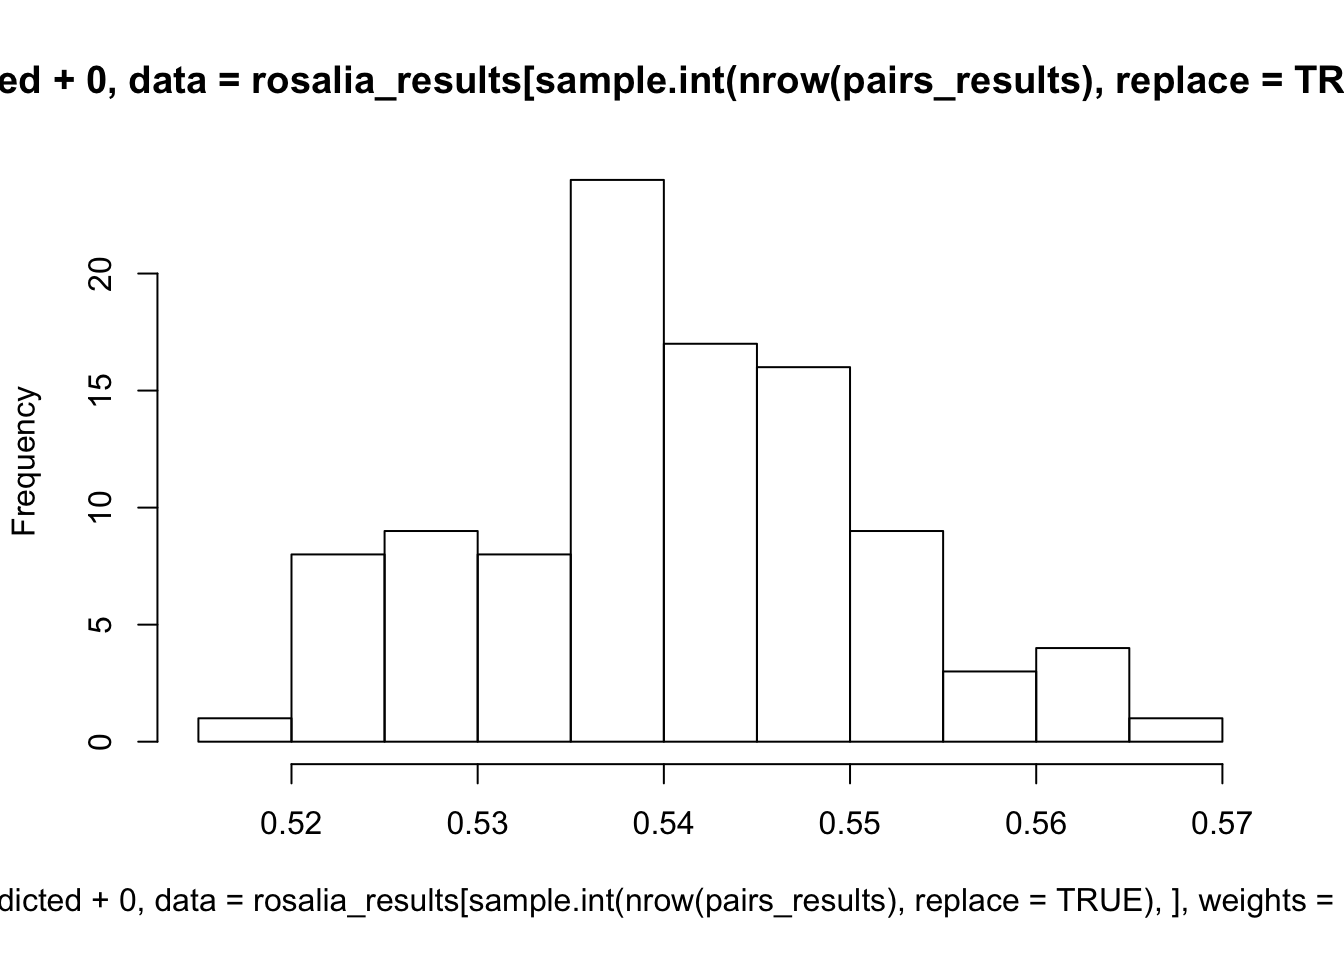
\includegraphics{show-results_files/figure-latex/unnamed-chunk-13-1.pdf}

\subsection{\texorpdfstring{Plot confidence interval coverage versus
true \(\beta\)
value}{Plot confidence interval coverage versus true \textbackslash{}beta value}}\label{plot-confidence-interval-coverage-versus-true-beta-value}

\begin{Shaded}
\begin{Highlighting}[]
\CommentTok{# Coverage versus true beta value.  The top and bottom 0.5%}
\CommentTok{# of the distribution have been omitted to prevent bad behavior}
\CommentTok{# by the smoother in the tails.}
\NormalTok{markov_summary %>%}
\StringTok{  }\KeywordTok{filter}\NormalTok{(}\KeywordTok{percent_rank}\NormalTok{(truth) >}\StringTok{ }\NormalTok{.}\DecValTok{005} \NormalTok{&}\StringTok{ }\KeywordTok{percent_rank}\NormalTok{(truth) <}\StringTok{ }\NormalTok{.}\DecValTok{995}\NormalTok{) %>%}
\StringTok{  }\KeywordTok{mutate}\NormalTok{(}\DataTypeTok{covered =} \NormalTok{truth >}\StringTok{ }\NormalTok{lower &}\StringTok{ }\NormalTok{truth <}\StringTok{ }\NormalTok{upper) %>%}
\StringTok{  }\KeywordTok{ggplot}\NormalTok{(}\KeywordTok{aes}\NormalTok{(}\DataTypeTok{x =} \NormalTok{truth, }\DataTypeTok{y =} \KeywordTok{as.integer}\NormalTok{(covered))) +}\StringTok{ }
\StringTok{  }\KeywordTok{facet_grid}\NormalTok{(~simulation_type) +}\StringTok{ }
\StringTok{  }\KeywordTok{geom_smooth}\NormalTok{(}\DataTypeTok{method =} \NormalTok{gam, }\DataTypeTok{formula =} \NormalTok{y ~}\StringTok{ }\KeywordTok{s}\NormalTok{(x), }\DataTypeTok{family =} \NormalTok{binomial) +}\StringTok{ }
\StringTok{  }\KeywordTok{theme_bw}\NormalTok{() +}\StringTok{ }
\StringTok{  }\KeywordTok{coord_cartesian}\NormalTok{(}\DataTypeTok{ylim =} \KeywordTok{c}\NormalTok{(}\DecValTok{0}\NormalTok{, }\DecValTok{1}\NormalTok{)) +}\StringTok{ }
\StringTok{  }\KeywordTok{geom_vline}\NormalTok{(}\DataTypeTok{xintercept =} \DecValTok{0}\NormalTok{) +}\StringTok{ }
\StringTok{  }\KeywordTok{geom_hline}\NormalTok{(}\DataTypeTok{yintercept =} \FloatTok{0.95}\NormalTok{, }\DataTypeTok{color =} \StringTok{"red"}\NormalTok{) +}\StringTok{ }
\StringTok{  }\KeywordTok{ylab}\NormalTok{(}\StringTok{"Coverage"}\NormalTok{)}
\end{Highlighting}
\end{Shaded}

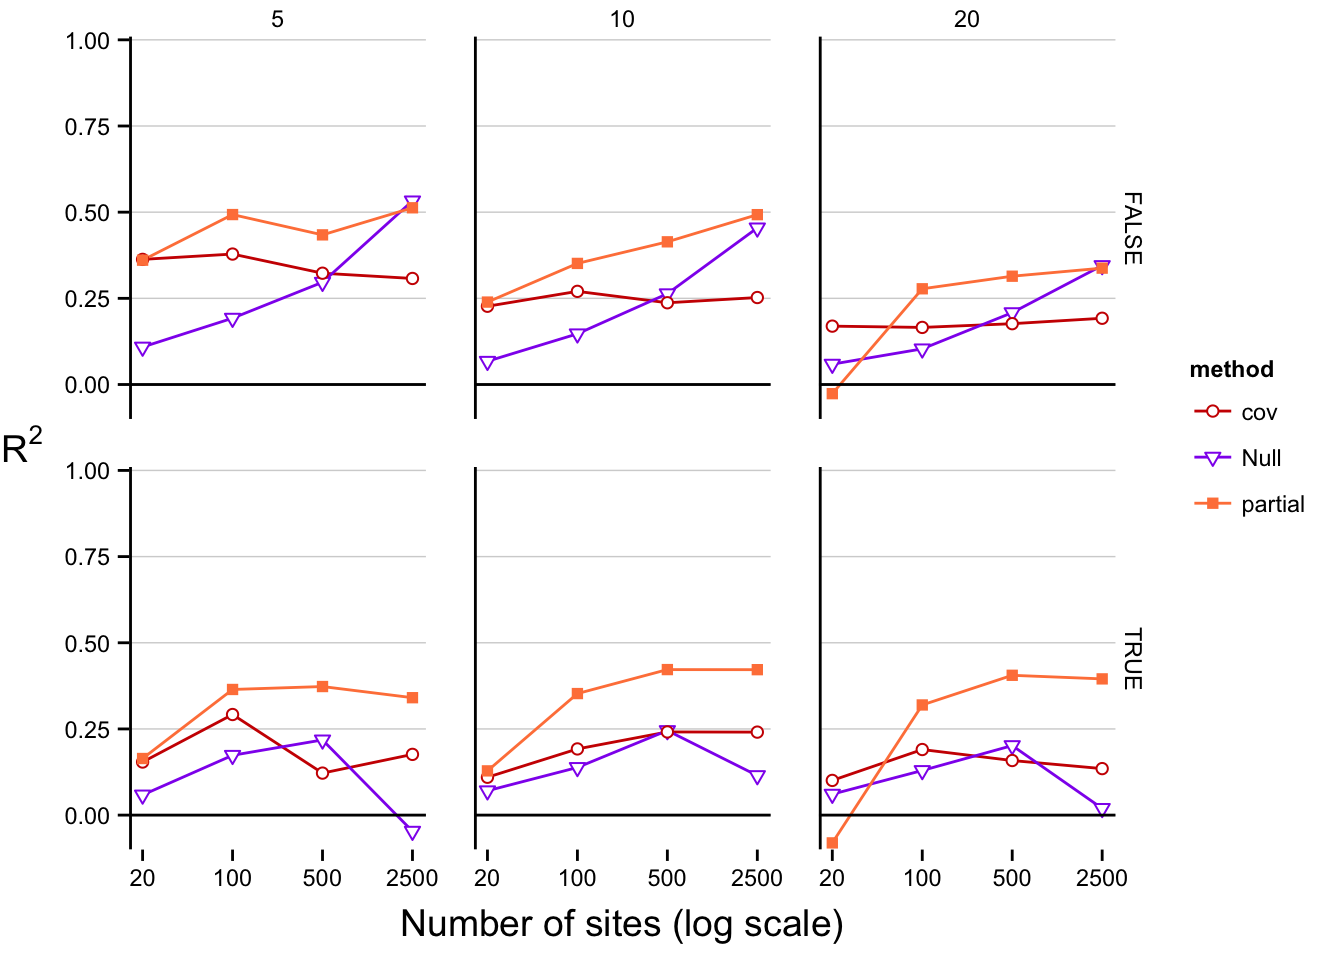
\includegraphics{show-results_files/figure-latex/unnamed-chunk-14-1.pdf}

\end{document}
